\documentclass[12pt]{article}

\usepackage{tema2014}

\usepackage{graphicx,url}

\usepackage[brazil]{babel}
\usepackage[utf8]{inputenc}


\sloppy

\title{Modelo de documento para as conferências da TeMA}

\author{Xxxxx Xxxxx\inst{1}, Xxxxx Xxxxx\inst{2}}

\address{Rua/Av. Xxxxxxxx, n. --- Município-UF --- CEP: xxxxx-xxx\\
  $^2$Rua/Av. Xxxxxxxx, n. --- Município-UF --- CEP: xxxxx-xxx\\
  \email{xxxx@xxxx.xxx, xxxx@xxxx.xxx}
}

\begin{document}

\maketitle

\begin{abstract}
  This meta-paper describes the style to be used in paper submission
  for the conferences of Associação Brasileira de Teoria e Análise
  Musical (TeMA).
\end{abstract}

\keywords{Template, TeMA, Music, Conference}

\begin{resumo}
  Este meta-artigo descreve o estilo a ser usado na elaboração de
  artigos para submissão nas conferências da Associação Brasileira de
  Teoria e Análise Musical (TeMA).
\end{resumo}

\palavraschave{Modelo, TeMA, Música, Congresso}

\section{Introdução}
\label{sec:gen}

Este modelo inclui toda a informação referente à formatação de artigos
para as conferências da TeMA. Este guia deverá ser seguido para que os
anais dos eventos tenham um padrão uniforme. Este modelo pode ser
obtido na página da TeMA (http://tema.mus.br).

\section{Formato do arquivo de entrega}
\label{sec:formato-arquivo}

O artigo deverá ser entregue unicamente em formato pdf. Este modelo
está disponível nos formatos tex, odt, doc e docx.

\subsection{Formatos odt, doc e docx}
\label{sec:formatos-odt-doc}

Os modelos em arquivos odt, doc e docx já têm estilos configurados
para o título, nomes de autores, abstract e resumo, títulos de seções
e subseções, corpo de texto, legendas de figuras e referências.
Recomendamos fortemente o uso da galeria de estilos para a elaboração
do documento (vide guia de estilos em \url{http://goo.gl/eviv}).

Antes de submeter o trabalho, o arquivo deverá ser convertido para o
formato pdf. Usuários de Windows poderão usar qualquer conversor, como
Adobe ou PDF Forge (\url{http://www.pdfforge.org/}). Linux e Mac já
têm o recurso de impressão para PDF nativamente instalado.

\subsection{Formato \LaTeX}
\label{sec:latex}

O modelo está disponível em \LaTeX{}. Neste modelo estão contidos o
estilo do artigo, o estilo da bibliografia e um script \textit{make}
para automação da compilação do arquivo pdf. O modelo está documentado
em \url{http://goo.gl/0aHgJU}.

\section{Tamanho da página}
\label{sec:tamanho-pagina}

Os anais serão organizados em formato A4 retrato (21.0cm x 29.7cm).
Todo o conteúdo de cada página deverá caber dentro do retângulo de
15cm x 23.7cm, centralizado na página, com margens de 3cm em todos os
lados. O texto deverá estar inteiramente justificado, com separação de
sílabas.

O artigo deverá ter um máximo de \textbf{10 páginas}, tanto na versão
de avaliação quanto na versão final, incluídos título, resumo e
abstract, palavras-chave e keywords, notas, referências e exemplos
(figuras, tabelas).

\section{Fonte}
\label{sec:fonte}

Todo o texto deverá ter fonte Times, exceto pelas legendas das figuras
(vide seção~\ref{sec:figuras-e-tabelas}). Fontes sem serifa e não
proporcional só podem ser usadas com propósitos especiais, como para
diferenciar texto de código-fonte de programas.

\section{Primeira página}

A primeira página deverá conter o título do artigo, o nome e endereço
dos autores, o abstract e \textit{keywords} em inglês, e, nos textos
em português, o resumo e palavras-chave.

\subsection{Título}
\label{sec:titulo}

O título deverá ser centralizado sobre a página, com fonte Times em
negrito 16pt. O espaçamento entre \textit{keywords} e resumo deverá
ser de 12pt.

\subsection{Autores}
\label{sec:autores}

O nome do autor (substituído por Xxxx na versão para submissão) deverá
 estar centralizado, com fonte Times 12pt, em negrito, com espaçamento
de 12pt antes e depois; Nomes de múltiplos autores devem estar disposto(s)
 consecutivamente e separados por vírgulas.

O endereço, profissional (substituído por Xxxxx na submissão), deverá
estar centralizado, com fonte Times 12pt, com espaçamento de 12pt antes
 e depois. No caso de múltiplas autorias, se o endereço for o mesmo,
 deverá ser inserido apenas uma vez, centralizado; endereços diferentes
 deverão ter espaçamento de 12pt antes e depois.

O e-mail (substituído por Xxxxx na versão para submissão) deverá estar
 centralizado, em fonte Courier 10pt, com espaçamento de 12pt antes e
depois. E-mails de múltiplos autores devem estar disposto(s) consecutivamente,
separados por vírgulas.


\subsection{Abstract e resumo}
\label{sec:abstract-e-resumo}

O abstract e o resumo deverão ter fonte Times itálico 12pt, em
itálico, indentado em 0.8cm em ambos os lados. O espaçamento entre
\textit{abstract}, \textit{keywords}, resumo e palavras-chave deverá
ser de 12pt.

O resumo deverá conter uma introdução, o objetivo do projeto
trabalhado, a metodologia, os resultados (parciais ou finais) e
apontar as conclusões. O resumo deverá ter, entre 150 e 300 palavras,
sem divisão em parágrafos e sem citações bibliográficas.

\subsection{\textit{Keywords} e palavras-chave}
\label{sec:keywords-e-palavras}

O texto deverá conter até 5 \textit{keywords} e palavras-chave
separadas por vírgula.

\section{Corpo do texto}

\subsection{Seções e subseções}
\label{sec:secoes}

Os títulos de seções e subseções deverão ser obrigatoriamente
enumerados, deverão ter fonte Times, negrito, 13pt e alinhamento à
esquerda. Deverá haver dois espaços entre a numeração e o título da
seção/subseção.

Títulos de seções e subseções deverão ser precedidos e sucedidos de
espaço extra. Em seções os títulos deverão ser precedidos por espaço
de 24pt, e em subseções, 12pt. Ambos deverão ser sucedidos por espaço
de 12pt.

\subsection{Parágrafos}
\label{sec:paragrafos}

O primeiro parágrafo de cada seção não deverá estar indentado. Os
seguintes deverão ter indentação 0.5cm. O espaçamento entre parágrafos
deverá ser de 3pt.

\subsection{Números de página, cabeçalhos e rodapés}

As páginas não deverão conter cabeçalhos, rodapés ou números de página
em sua submissão. Estes elementos serão adicionados quando os anais
forem confeccionados.

\subsection{Notas de rodapé}

As notas de rodapé deverão ser identificadas com um número no texto e
inseridas na base da página em que aparecem\footnote{Este é um exemplo
  de nota de rodapé.}. As notas deverão ter fonte de 10pt e deverão ser
precedidas de linha horizontal de 0.5pt.

\section{Figuras e tabelas}
\label{sec:figuras-e-tabelas}

As figuras e tabelas deverão ser, preferencialmente, flutuantes,
ocorrendo no topo da página em que são mencionadas ou da página
seguinte. Figuras e tabelas deverão ser enumeradas
\textbf{independentemente} e referendadas por seus números (por
exemplo, figura~\ref{fig:exampleFig}).

\begin{figure}
\centering
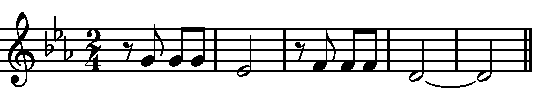
\includegraphics[width=.5\textwidth]{beethoven}
\caption{Uma figura típica}
\label{fig:exampleFig}
\end{figure}

As legendas das figuras e tabelas, se menores que uma linha, deverão
ser centralizadas. Nos outros casos, deverão ser justificadas e
indentadas em 0.8cm em ambos lados. A fonte deverá ser Helvetica
negrito, de 10pt, com 6pt de espaço antes e depois de cada legenda.

Nas tabelas, não usar fundo colorido ou sombreado e evitar linhas
grossas, duplas ou desnecessárias.


\section{Imagens}

Todas as imagens e ilustrações deverão estar em preto e branco ou tons
de cinza. A resolução das imagens deverá ser de até 600 dpi para preto
e branco e 200 dpi para tons de cinza. Não incluir imagens com
resolução excessiva.

\section{Referências}

Referências bibliográficas deverão ser uniformes, com o sistema
Turabian autor data. Por exemplo, \cite{kroger04:desenvolvendo},
\cite{babbitt61:set}, \cite{coutinho.ea05:computational},
\cite{morris87:composition}. Não deverá haver espaçamento entre
linhas. O texto deverá ter recuo de 0,75cm, exceto a primeira linha.

\bibliography{references}

\end{document}
